\documentclass[aspectratio=169]{beamer}
\makeatletter
\def\input@path{{../common/}{../guide/}{../data/}{../code/}}
\makeatother
\usetheme{Bruno}
\input{preamble}
\title{Transductores: Conceptos básicos}
\author{
    Eduardo Font y Juan J. Rojas
}
\institute{Instituto Tecnológico de Costa Rica}
\date{\today}
\background{background.jpg}
\begin{document}
\input{postamble}
\maketitle

\newcommand{\blackandwhite}{white} %change this at the end

\begin{frame}{Señales}
    \begin{columns}[c, onlytextwidth]
        \begin{column}{0.6\textwidth}
        Una \textbf{señal} es la representación de una medición de una magnitud física que varía con una o más variables independientes y que porta información relevante.\\[8pt]
        Características: 
            \begin{itemize}
                \item Escalar o vectorial 
                \item Discreta o continua
                \item Determinista o aleatoria
            \end{itemize}    
        \end{column}
        \begin{column}{0.4\textwidth}
            \begin{center}
                \begin{tikzpicture}
                    \begin{axis}[
                        width= 0.9\linewidth,
                        height= 0.6\linewidth,
                        domain=0:4*pi,
                        samples=100,
                        ymin=-1.2, ymax=1.2,
                        xmin=0, xmax=4*pi+0.5,
                        axis x line=center,
                        axis y line=left,
                        ytick={\empty},
                        yticklabels={\empty},
                        xtick={\empty},
                        xticklabels={\empty},
                        %xtick={pi,2*pi,3*pi,4*pi},
                        %xticklabels={$\pi$,$2\pi$,$3\pi$,$4\pi$},
                        xlabel=$t$, % Set the labels
                        ylabel=$f(t)$,
                        x unit=, 
                        y unit=,
                        axis lines=center,
                        x label style={anchor=west},
                        y label style={anchor=south},
                        ]
                        \addplot[color=blue,mark=none,thick] {sin(deg(x))}
                    	;
                    \end{axis}
                    \begin{axis}[
                        yshift=-3cm,
                        width= 0.9\linewidth,
                        height= 0.6\linewidth,
                        domain=0:4*pi,
                        samples=100,
                        ymin=-1.2, ymax=1.2,
                        xmin=0, xmax=4*pi+0.5,
                        axis x line=center,
                        axis y line=left,
                        ytick={\empty},
                        yticklabels={\empty},
                        xtick={\empty},
                        xticklabels={\empty},
                        %xtick={pi,2*pi,3*pi,4*pi},
                        %xticklabels={$\pi$,$2\pi$,$3\pi$,$4\pi$},
                        xlabel=$p$, % Set the labels
                        ylabel=$f(p)$,
                        x unit=, 
                        y unit=,
                        axis lines=center,
                        x label style={anchor=west},
                        y label style={anchor=south},
                        ]
                        \addplot[color=red,mark=none,thick] {rand}
                    	;
                    \end{axis}
                \draw[\blackandwhite] (-0.5,-3.2) rectangle (4,2.5);
                \end{tikzpicture}
            \end{center}
        \end{column}
    \end{columns}
\end{frame}

\begin{frame}{Estímulos}
Magnitud física, del entorno o del sistema en estudio, que actúa sobre un sensor y que puede ser medida para generar una señal.\\[8pt]
Algunos ejemplos de estímulos: 
    \begin{itemize}
        \item Aceleración 
        \item Intensidad de radiación
        \item Temperatura
        \item Concentración de un componente químico
    \end{itemize}    
\end{frame}

\begin{frame}{Sistemas}
    \begin{columns}[c, onlytextwidth]
        \begin{column}{0.4\textwidth}
        Un sistema es una construcción o colección de diferentes elementos que juntos producen resultados que no pueden obtenerse con los elementos por separado\cite{INCOSE}.\\[8pt]
        Un sistema es un objeto o conjunto de objetos cuyas propiedades queremos estudiar\cite{modelica}.
        \end{column}
        \begin{column}{0.6\textwidth}
            \begin{center}
               \includegraphics[width=\textwidth]{01_intro/tostadora.jpg}\\
               \tiny{Tomado de \href{https://deseng.ryerson.ca/dokuwiki/_detail/design:toasterarchitecture.jpg?id=design\%3Asystem_diagram}{aquí}}
            \end{center}
        \end{column}
    \end{columns}
\end{frame}

\begin{frame}{Señales de entrada y salida}
    \begin{columns}[c, onlytextwidth]
        \begin{column}{0.4\textwidth}
             \begin{itemize}
                \item Entradas: son las variables que afectan el comportamiento del sistema
                \item Salidas: son las variables que son definidas por el sistema
             \end{itemize}
        \end{column}
        \begin{column}{0.6\textwidth}
            \begin{center}
               \includegraphics[width=\textwidth]{01_intro/tostadora.jpg}\\
               \tiny{Tomado de \href{https://deseng.ryerson.ca/dokuwiki/_detail/design:toasterarchitecture.jpg?id=design\%3Asystem_diagram}{aquí}}
            \end{center}
        \end{column}
    \end{columns}
\end{frame}

\begin{frame}{Modelos y simulaciones}
    \begin{columns}[c, onlytextwidth]
        \begin{column}{0.5\textwidth}
        Un modelo es una abstracción matemática de un sistema.\\[8pt]
        \begin{itemize}
            \item Se modela el sistema en base a ecuaciones
            \item Es una simplificación del sistema real
            \item Solo es valido en ciertas condiciones y/o rangos
        \end{itemize}
        Una simulación es un experimento que se realiza en el modelo de un sistema.
        
        \end{column}
        \begin{column}{0.5\textwidth}
            \begin{center}
                \begin{circuitikz}
                    \draw 
                    (0,0)
                        to[cV, l=$OCV(z)$]
                    (0,3)
                        to[R, l=$R_0$,i=$i(t)$,-o]
                    (3,3)
                        to[open,v^=$v(t)$]
                    (3,0)
                        to[short,o-]
                    (0,0)
                    ;
                \end{circuitikz}\\[8pt]
                \footnotesize{Modelo Rint de una celda electroquímica}
            \end{center}
        \end{column}
    \end{columns}
\end{frame}

\begin{frame}{Transductores, sensores y actuadores}
    \begin{columns}[c, onlytextwidth]
        \begin{column}{0.6\textwidth}
        Para los efectos de este curso...\\[8pt]
        \begin{itemize}
            \item \textbf{Transductor:} dispositivo que convierte una señal de un tipo de energía a una señal correspondiente pero con un tipo de energía diferente.
            \item \textbf{Sensor:} transductor que convierte una señal física a un señal eléctrica
            \item \textbf{Actuador:} transductor que convierte una señal eléctrica a un señal física
        \end{itemize}
        \end{column}
        \begin{column}{0.4\textwidth}
            \begin{center}
               \includegraphics[width=0.8\textwidth]{presion/bourdon.png}\\
               \tiny{Tomado de \href{https://upload.wikimedia.org/wikipedia/commons/thumb/7/74/MAXIMATOR-High-Pressure-Manometer-01a.jpg/1200px-MAXIMATOR-High-Pressure-Manometer-01a.jpg}{aquí}}
            \end{center}
        \end{column}
    \end{columns}
\end{frame}

\begin{frame}{Sensores directos y complejos}
    \begin{columns}[c, onlytextwidth]
        \begin{column}{0.5\textwidth}
        Sensor directo
            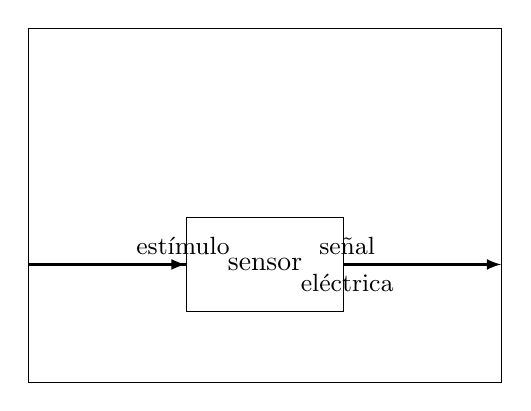
\begin{tikzpicture}
                \node[draw,minimum width=2cm,minimum height=1.2cm](sensor) {sensor};
                \draw[>=latex, thick, ->](sensor) --++ (-3,0) -- (sensor);
                \node[left=1,above] at (sensor.west){\small estímulo};
                \draw[>=latex, thick, ->](sensor) -- (sensor) --++ (3,0);
                \node[right=1,above] at (sensor.east){\small señal};
                \node[right=1,below] at (sensor.east){\small eléctrica};
                \draw[\blackandwhite] (-3,-1.5) rectangle (3,3);
            \end{tikzpicture}
        \end{column}
        \begin{column}{0.5\textwidth}
        Sensor complejo
            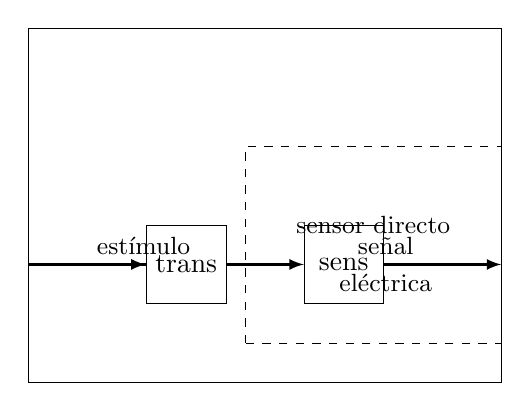
\begin{tikzpicture}
            \node[draw,minimum width=1cm,minimum height=1cm](s1) {trans};
            \draw[>=latex, thick, ->](s1) --++ (-2,0) -- (s1);
            \node[left=0.75,above] at (s1.west){\small estímulo};
            \node[draw,minimum width=1cm,minimum height=1cm,right of=s1,node distance=2cm](s2) {sens};
            \draw[>=latex, thick, ->](s2) -- (s2) --++ (2,0);
            \node[right=0.75,above] at (s2.east){\small señal};
            \node[right=0.75,below] at (s2.east){\small eléctrica};
            \draw[>=latex, thick, ->](s1) -- (s2);
            \draw[\blackandwhite] (-2,-1.5) rectangle (4,3);
            \draw[black, dashed] (0.75,-1) rectangle (4,1.5)node[midway,above=0.7]{\small sensor directo};
            \end{tikzpicture}
        \end{column}
    \end{columns}
\end{frame}

\begin{frame}{Sensores pasivos y activos}
    \begin{columns}[c, onlytextwidth]
        \begin{column}{0.5\textwidth}
        Sensor pasivo
            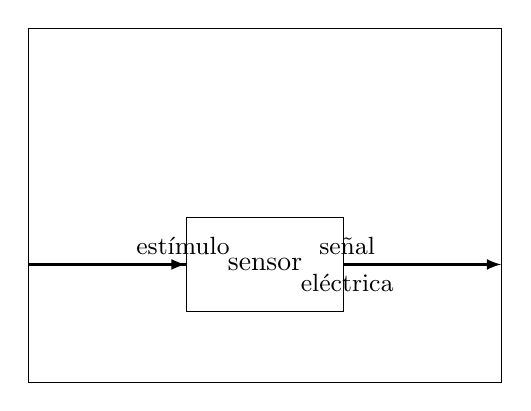
\begin{tikzpicture}
                \node[draw,minimum width=2cm,minimum height=1.2cm](sensor) {sensor};
                \draw[>=latex, thick, ->](sensor) --++ (-3,0) -- (sensor);
                \node[left=1,above] at (sensor.west){\small estímulo};
                \draw[>=latex, thick, ->](sensor) -- (sensor) --++ (3,0);
                \node[right=1,above] at (sensor.east){\small señal};
                \node[right=1,below] at (sensor.east){\small eléctrica};
                \draw[\blackandwhite] (-3,-1.5) rectangle (3,3);
            \end{tikzpicture}
        \end{column}
        \begin{column}{0.5\textwidth}
        Sensor activo
            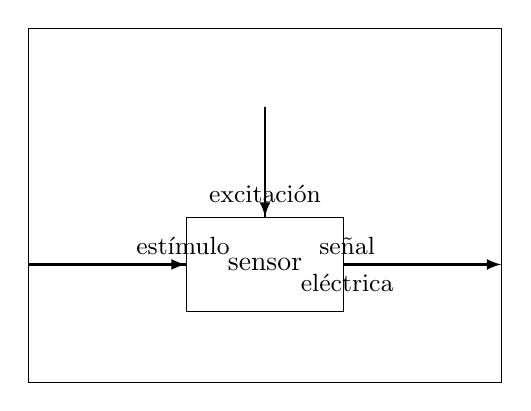
\begin{tikzpicture}
                \node[draw,minimum width=2cm,minimum height=1.2cm](sensor) {sensor};
                \draw[>=latex, thick, ->](sensor) --++ (-3,0) -- (sensor);
                \node[left=1,above] at (sensor.west){\small estímulo};
                \draw[>=latex, thick, ->](sensor) -- (sensor) --++ (3,0);
                \node[right=1,above] at (sensor.east){\small señal};
                \node[right=1,below] at (sensor.east){\small eléctrica};
                \draw[>=latex, thick, ->](sensor) --++ (0,+2) -- (sensor);
                \node[above=1.5] at (sensor.north){\small excitación};
                \draw[\blackandwhite] (-3,-1.5) rectangle (3,3);
            \end{tikzpicture}
        \end{column}
    \end{columns}
\end{frame}

\begin{frame}{Rangos de entrada y sálida, sesgo de sensado}
    \begin{columns}[c, onlytextwidth]
        \begin{column}{0.50\textwidth}
            \begin{itemize}
                \item Rango del estímulo (span): representa la diferencia entre el valor mínimo y el valor máximo del estímulo que pueden medirse con un error aceptable.
                \item Salida a escala completa (full-scale output, FSO): representa la diferencia entre los valores de la señal de salida que corresponden al valor mínimo y máximo del estímulo medido. 
            \end{itemize}
        \end{column}
        \begin{column}{0.45\textwidth}
            \textbf{Ejemplo}\\[4pt]
            Marca: Amphenol\\[4pt]
            Modelo: NovaSensor NPI-19\\[4pt]
            Estímulo: presión\\[4pt]
            Tipo: piezoresistivo\\[4pt]
            Rango del estímulo: $0  - \SI{17.2}{\kilo\pascal}$\\[4pt]
            Salida a escala completa: $\SI{125}{\milli\volt}$\\[4pt]
            Sesgo de sensado: $\pm \SI{1}{\milli\volt}$\\[10pt]
            \tiny{Tomado de \href{https://f.hubspotusercontent40.net/hubfs/9035299/Documents/AAS-920-298B-NovaSensor\%20NPI-19-REVISED-061714-web.pdf}{aquí}}
        \end{column}
    \end{columns}
\end{frame}

\begin{frame}{Sesgo de sensado e histeresis}
    \begin{columns}[c, onlytextwidth]
        \begin{column}{0.50\textwidth}
            \begin{itemize}
                \item Sesgo de sensado (offset): es el rango de valores de la señal de salida cuando el estimulo tiene valor cero. 
                \item Histéresis: es una desviación de la señal de salida  que se obtiene al realizar la medición de un mismo valor de un estímulo en direcciones opuestas.
            \end{itemize}
        \end{column}
        \begin{column}{0.45\textwidth}
            \textbf{Ejemplo}\\[4pt]
            Marca: Allen-Bradley\\[4pt]
            Modelo: 875C AC\\[4pt]
            Estímulo: posición\\[4pt]
            Tipo: capacitivo\\[4pt]
            Histéresis: $\leq 10 \%$\\[10pt]
            \tiny{Tomado de \href{https://literature.rockwellautomation.com/idc/groups/literature/documents/td/875-td001_-en-p.pdf}{aquí}}
        \end{column}
    \end{columns}
\end{frame}

\begin{frame}{Exactitud y precisión}
    \begin{columns}[c, onlytextwidth]
        \begin{column}{0.55\textwidth}
            \begin{itemize}
                \item Valor real de un estimulo: es el que se obtendría con una medición perfecta. Sin embargo este valor es indeterminado y por lo tanto se define por algún tipo de convención. 
                \item Exactitud: es la capacidad de un sensor de dar un resultado cercano al valor real del estímulo medido.
                \item Precisión: es la capacidad de un sensor de dar el mismo resultado cuando se mide el mismo valor de un estimulo bajo las mismas condiciones. 
            \end{itemize}
        \end{column}
        \begin{column}{0.40\textwidth}
            \textbf{Ejemplo}\\[4pt]
            Marca: Amphenol\\[4pt]
            Modelo: NovaSensor NPI-19\\[4pt]
            Estímulo: presión\\[4pt]
            Tipo: piezoresistivo\\[4pt]
            Exactitud estática$^*$: $0.1 \%$ \\[10pt]
            % Exactitud térmica del FSO: $\pm 0.5 \% $\\[4pt]
            % Exactitud térmica del offset: $\pm 0.5 \% $\\[10pt]
            \tiny{* Incluye errores de linealidad, histéresis y repetibilidad}\\
            \tiny{Tomado de \href{https://f.hubspotusercontent40.net/hubfs/9035299/Documents/AAS-920-298B-NovaSensor\%20NPI-19-REVISED-061714-web.pdf}{aquí}}
        \end{column}
    \end{columns}
\end{frame}

\begin{frame}{Repetibilidad y reproducibilidad}
    \begin{columns}[c, onlytextwidth]
        \begin{column}{0.60\textwidth}
            \begin{itemize}
                \item Repetibilidad: es una medida de la proximidad de la concordancia entre dos mediciones del mismo valor de un estímulo realizadas por la misma persona, con el mismo método e instrumento, bajo las mismas condiciones y en un periodo corto de tiempo. 
                \item Reproducibilidad: es una medida del grado de concordancia entre dos mediciones del mismo valor de un estímulo realizadas por diferentes personas, con el mismo método, con diferentes instrumentos y en un periodo largo de tiempo. 
            \end{itemize}
        \end{column}
        \begin{column}{0.35\textwidth}
            \includegraphics[width=0.9\textwidth]{repeatibility.png}\cite{Fraden_2016}
            \begin{equation*}
                \delta_r = \dfrac{\Delta}{FS}\cdot 100\%
            \end{equation*}
        \end{column}
    \end{columns}
\end{frame}

\begin{frame}{Linealidad y resolución}
    \begin{columns}[c, onlytextwidth]
        \begin{column}{0.55\textwidth}
            \begin{itemize}
                \item Linealidad: es una medida de la proximidad entre la curva de calibración (valores medidos) y una linea recta específica.
                \item Resolución: es el incremento mas pequeño en el valor del estimulo que puede ser medido por el sensor. 
            \end{itemize}
        \end{column}
        \begin{column}{0.40\textwidth}
            \textbf{Ejemplo}\\[4pt]
            Marca: PIHER\\[4pt]
            Modelo: PS2P-LIN\\[4pt]
            Estímulo: posición\\[4pt]
            Tipo: magnetico, efecto Hall\\[4pt]
            Rango del estímulo: $\SI{12}{\milli\meter}$\\[4pt]
            Salida a escala completa (PWM): $10\% (\SI{-6}{\milli\meter}) \sim 90\% (\SI{6}{\milli\meter})$\\[4pt]
            Linealidad: $\pm 1 \%$ \\[4pt]
            Resolución(PWM): $14\,\mathrm{bits}$\\[10pt]
            \tiny{Tomado de \href{https://www.piher.net/products/contactless-position-sensors/linear-position-sensors/hall-effect-linear-position-sensors/ps2p-lin/}{aquí}}
        \end{column}
    \end{columns}
\end{frame}


\begin{frame}{Sensibilidad, saturación y banda muerta}
    \begin{columns}[c, onlytextwidth]
        \begin{column}{0.60\textwidth}
            \begin{itemize}
                \item Sensibilidad: es la pendiente de la curva de calibración, sin importar si es constante o no en todo el rango de salida.  
                \item Saturación: es el rango de operación en el que un incremento en el valor del estímulo no produce variaciones en la señal de salida del sensor. 
                \item Banda muerta: es el rango de operación en el que, sin importar el valor del estímulo, la salida es cercana a cero.
            \end{itemize}
        \end{column}
        \begin{column}{0.35\textwidth}
            \textbf{Ejemplo}\\[4pt]
            Marca: Allegro\\[4pt]
            Modelo: ACS723\\[4pt]
            Estímulo: corriente eléctrica\\[4pt]
            Tipo: magnetico, efecto Hall\\[4pt]
            Rango del estímulo: $\SI{10}{\ampere}$\\[4pt]
            Salida a escala completa: $\SI{0.5}{\volt}(\SI{-5}{\ampere}) \sim \SI{4.5}{\volt}(\SI{5}{\ampere})$\\[4pt]
            Sensibilidad: $\SI{400}{\milli\volt/\ampere}$ \\[4pt]
            Saturación: $<\SI{0.5}{\volt}, >\SI{4.5}{\volt}$\\[10pt]
            \tiny{Tomado de \href{https://www.allegromicro.com/-/media/files/datasheets/acs723-datasheet.ashx}{aquí}}
        \end{column}
    \end{columns}
\end{frame}

\begin{frame}{Valor real, error absoluto y relativo}
    \begin{columns}[c, onlytextwidth]
        \begin{column}{0.55\textwidth}
            \begin{itemize}
                \item Valor real: es el valor de salida que se obtendría con una medición perfecta. Debido a que esto es imposible de determinar se utiliza una convención para definir el valor real.  
                \item Error absoluto: es la diferencia entre una medición y el valor real. 
                \item Error relativo: es el cociente entre el error absoluto y el valor real
            \end{itemize}
        \end{column}
        \begin{column}{0.40\textwidth}
            \begin{equation*}
                \mathrm{error\,absoluto} = \mathrm{medición} - \mathrm{valor\,real}
            \end{equation*}
            \begin{equation*}
                \mathrm{error\,relativo} = \dfrac{\mathrm{error\,absoluto}}{\mathrm{valor\,real}}
            \end{equation*}
        \end{column}
    \end{columns}
\end{frame}

\begin{frame}{Sistemas de magnitudes y unidades: SMU -- ISQ -- SI}
    \begin{columns}[c, onlytextwidth]
        \begin{column}{0.65\textwidth}
            \begin{itemize}
                \item Un \textbf{sistema de magnitudes y unidades (SMU)} organiza magnitudes físicas, dimensiones y unidades de medida.
                \item El \textbf{ISQ} (International System of Quantities) define magnitudes base y derivadas para describir fenómenos físicos de forma coherente.
                \item El \textbf{SI} asigna unidades a esas magnitudes: metro, kilogramo, segundo, ampere, kelvin, mol y candela.
                \item Una unidad derivada coherente se obtiene directamente de unidades base, por ejemplo:
            \end{itemize}
            \[
                F = m a
                \;\Rightarrow\;
                1\,\si{\newton} = 1\,\si{\kilogram\meter\per\second\squared}
            \]
        \end{column}
        \begin{column}{0.50\textwidth}
            \small
            \begin{tabular}{lll}
                \textbf{Magnitud} & \textbf{Unidad} & \textbf{Sím.} \\
                Longitud & metro & m \\
                Masa & kilogramo & kg \\
                Tiempo & segundo & s \\
                Corriente & ampere & A \\
                Temperatura & kelvin & K \\
                Cantidad de sustancia & mol & mol \\
                Intensidad luminosa & candela & cd \\
            \end{tabular}\\[8pt]
            \tiny{Basado en \cite{isq_iso80000_1,bipm_si_2019}.}
        \end{column}
    \end{columns}
\end{frame}

\begin{frame}{Simbología de instrumentos: normas ANSI/ISA}
    \begin{columns}[c, onlytextwidth]
        \begin{column}{0.56\textwidth}
            \begin{itemize}
                \item La norma \textbf{ANSI/ISA-5.1} estandariza símbolos e identificación de instrumentos en diagramas P\&ID.
                \item Las letras del \textbf{tag} describen variable medida y función del instrumento.
                \item Esto mejora comunicación entre diseño, operación y mantenimiento.
            \end{itemize}
            \vspace{6pt}
            \textbf{Ejemplos de tags}\\[4pt]
            \begin{itemize}
                \item \textbf{PT-101}: transmisor de presión.
                \item \textbf{TIC-203}: controlador indicador de temperatura.
                \item \textbf{FV-210}: válvula de control de flujo.
            \end{itemize}
        \end{column}
        \begin{column}{0.40\textwidth}
            \small
            \begin{tabular}{ll}
                \textbf{Letra} & \textbf{Significado} \\
                P & Presión \\
                T (1ra letra) & Temperatura \\
                F & Flujo \\
                L & Nivel \\
                I & Indicador \\
                T (2da letra) & Transmisor \\
                C & Controlador \\
                V & Válvula \\
            \end{tabular}\\[10pt]
            \tiny{Referencia: \cite{ansi_isa_5_1}.}
        \end{column}
    \end{columns}
\end{frame}


\begin{frame}{Referencias}
\footnotesize
\printbibliography[heading=none]
\end{frame}


\end{document}
